\section{KHOẢNG CÁCH}

\subsection{PHÂN LOẠI, PHƯƠNG PHÁP GIẢI TOÁN}
\begin{dang}{Khoảng cách từ một điểm tới một đường thẳng}
	\immini{
		Để tính khoảng cách từ điểm $O$ tới đường thẳng $d$, ta thực hiện các bước sau:
		\begin{itemize}
			\item Trong mặt phẳng $(O;d)$, hạ $OH \perp d$ tại $H$.
			\item Suy ra $\mathrm{d}\left(O,d \right)=OH.$ 
		\end{itemize}
	}{
		\begin{tikzpicture}[scale=1, font=\footnotesize, line join=round, line cap=round,>=stealth]
			\tkzInit[xmin=-2,xmax=4,ymin=-0.5,ymax=2.5] 
			\tkzClip
			\tkzDefPoints{-2/0/A, 3/0/B, 0/1.5/O}
			\tkzDrawSegments(A,B)		
			\tkzDrawAltitude(A,B)(O)\tkzGetPoint{H}
			\tkzDrawPoints[fill=black](O,H)
			\tkzLabelPoints[above](O)
			\tkzLabelPoints[below](H)
			\tkzMarkRightAngles(B,H,O)
			\tkzLabelSegment[above,pos=0.9](A,B){$d$}		
		\end{tikzpicture}
	}
\end{dang}

\begin{vd}
	\immini{Cho hình chóp $S.ABCD$ có đáy $ABCD$ là hình vuông cạnh $a$, tâm $O$, $SA=a$ và vuông góc với mặt phẳng $(ABCD)$. Gọi $I, M$ theo thứ tự là trung điểm của $SC, AB$.
	\begin{tasks}(1)
		\task Chứng minh $OI \perp (ABCD)$.
		\task Tính khoảng cách từ $I$ đến $CM$, từ đó suy ra khoảng cách từ $S$ tới $CM$.
	\end{tasks}}{
\begin{tikzpicture}[scale=1, font=\footnotesize, line join=round, line cap=round,>=stealth]
	\tkzDefPoints{0/0/A, -2/-2/B, 3/-2/C}
	\coordinate (D) at ($(A)+(C)-(B)$);
	\coordinate (S) at ($(A)+(0,3)$);
	\tkzInterLL(A,C)(B,D)\tkzGetPoint{O}
	\tkzDefMidPoint(B,A)\tkzGetPoint{M}
	\tkzDefMidPoint(S,C)\tkzGetPoint{I}
	\tkzInterLL(M,C)(B,O)\tkzGetPoint{K}
	\coordinate (H) at ($(K)!0.25!(C)$);
	\tkzDrawPolygon(S,C,D)
	\tkzDrawSegments(S,B B,C)
	\tkzDrawSegments[dashed](S,A A,B A,D A,C B,D O,I C,M)
	\tkzDrawPoints[size=4,fill=black](A,B,C,D,S,I,O,K,M)
	\tkzLabelPoints[left](B)
	\tkzLabelPoints[right](C,D)
	\tkzLabelPoints[above](S,I,M,K)
	\tkzLabelPoints[above right](O,A)
	\tkzMarkRightAngle[size=0.15](K,O,C)
\end{tikzpicture}}
	\loigiai{
		
		\begin{enumerate}
			\immini{
				\item $OI$ là đường trung bình nên $OI \parallel SA$.\\
				Mặt khác $SA \perp (ABCD)$ nên  $OI \perp (ABCD)$.
				\item \indamm{Khoảng cách từ $I$ đến $CM$:}\\
				Kẻ $IH \perp CM$ tại $H$. Ta có 
				$$\heva{&CM \perp IH\\& CM \perp IO}\Rightarrow CM \perp OH.$$
				Suy ra $OH$ là đường cao trong tam giác vuông $OKC$, với $K=CM \cap BO$ là trọng tâm tam giác $ABC$. Ta tính được 
				$$OB=\dfrac{AC}{2}=\dfrac{a \sqrt 2}{2} \Rightarrow OK = \dfrac{OB}{3}=\dfrac{a \sqrt 2}{6}.$$
			}{
				\begin{tikzpicture}[scale=1, font=\footnotesize, line join=round, line cap=round,>=stealth]
					\tkzDefPoints{0/0/A, -2/-2/B, 3/-2/C}
					\coordinate (D) at ($(A)+(C)-(B)$);
					\coordinate (S) at ($(A)+(0,3)$);
					\tkzInterLL(A,C)(B,D)\tkzGetPoint{O}
					\tkzDefMidPoint(B,A)\tkzGetPoint{M}
					\tkzDefMidPoint(S,C)\tkzGetPoint{I}
					\tkzInterLL(M,C)(B,O)\tkzGetPoint{K}
					\coordinate (H) at ($(K)!0.25!(C)$);
					\tkzDrawPolygon(S,C,D)
					\tkzDrawSegments(S,B B,C)
					\tkzDrawSegments[dashed](S,A A,B A,D A,C B,D O,I C,M I,H O,H)
					\tkzDrawPoints[size=4,fill=black](A,B,C,D,S,I,O,K,M,H)
					\tkzLabelPoints[left](B)
					\tkzLabelPoints[right](C,D)
					\tkzLabelPoints[above](S,I,M,K)
					\tkzLabelPoints[above right](O,A)
					\tkzLabelPoints[below](H)	
					\tkzMarkRightAngle[size=0.15](K,O,C)
					\tkzMarkRightAngle[size=0.15](I,H,C)
				\end{tikzpicture}
			}
			Xét $\triangle OCK$ vuông tại $O$, có $\dfrac{1}{OH^2}=\dfrac{1}{OK^2}+\dfrac{1}{OC^2} \Rightarrow OH=\dfrac{OK \cdot OC}{\sqrt{OK^2+OC^2}}=\dfrac{a}{\sqrt{20}}$.\\
			Xét $\triangle OIH $ vuông tại $O$, có $IH^2=OI^2+OH^2 \Rightarrow IH=\dfrac{a\sqrt{30}}{10}$. Vậy $\mathrm{d}(I,CM)=IH=\dfrac{a\sqrt{30}}{10}$.\\
			\indamm{Khoảng cách từ $S$ đến $CM$:}\\
			Ta có $SI \cap CM=C$ và $\dfrac{CS}{CI}=2$ nên  $\dfrac{\mathrm{d}(S, CM)}{\mathrm{d}(I, CM)}=\dfrac{SC}{IC}=2 \Rightarrow \mathrm{d}(S, CM)=2\mathrm{d}(I, CM)=\dfrac{a\sqrt{30}}{{5}}$.
		\end{enumerate}
	}	
\end{vd}\dongcham{17}

\begin{vd}
	\immini{Cho hình chóp $S.MNPQ$ có đáy là hình thoi cạnh $a$, $SM$ vuông góc với mặt phẳng $(MNPQ)$, $SM = a\sqrt{3}$ và góc $\widehat{MNP} = 60^\circ$.
		\begin{tasks}(1)
			\task Chứng minh rằng $NQ \perp SP$.
			\task Tính khoảng cách giữa hai đường thẳng $MN$ và $PQ$.
			\task Gọi $H$ là hình chiếu vuông góc của $M$ lên $(SPQ)$. Tính độ dài $MH$.
		\end{tasks}
	}{
		\begin{tikzpicture}[scale=0.9, line join=round, line cap=round]
			\tkzDefPoints{0/0/M,-1.3/-1.6/N,2.5/-1.6/P}
			\coordinate (Q) at ($(M)+(P)-(N)$);
			\coordinate (S) at ($(M)+(0,3)$);
			%\coordinate (K) at ($(P)!0.5!(Q)$);
			%\coordinate (I) at ($(S)!0.45!(K)$);
			\tkzDrawPolygon(S,N,P,Q)
			\tkzDrawSegments(S,P)
			\tkzDrawSegments[dashed](M,N M,Q M,S M,P N,Q)
			\tkzDrawPoints[fill=black,size=4](S,M,N,P,Q)
			\tkzLabelPoints[above](S)
			\tkzLabelPoints[below](N,P)
			\tkzLabelPoints[right](Q)
			%	\tkzLabelPoints[below right](K)
			\tkzLabelPoints[left](M)
			%	\tkzMarkRightAngle[size=0.2](M,K,P)
			%	\tkzMarkRightAngle[size=0.2](M,I,K)
	\end{tikzpicture}}
	\loigiai{
		\begin{enumerate}
			\immini{\item Ta có $\heva{&NQ \perp MP \hspace{1cm}\text{(đường chéo hình thoi)} \\&NQ \perp SM \hspace{1cm}\text{(vì $SM \perp (MNPQ)$)} \\&MP,SM \subset (SMP)}$\\
				$\Rightarrow NQ \perp (SMP) \Rightarrow NQ \perp SP$.
				\item Ta có $MN \parallel PQ$ nên $\mathrm{d}(MN,PQ)=\mathrm{d}(M,PQ)$.\\
				Gọi $K$ là trung điểm của $PQ$. Do tam giác $MPQ$ đều nên $MK \perp PQ \Rightarrow \mathrm{d}(M,PQ)=MK$.\\
				$MK$ là đường cao trong tam giác đều nên $MK=\dfrac{a\sqrt{3}}{2}$.\\
				Vậy $\mathrm{d}(MN,PQ)=\mathrm{d}(M,PQ)=MK=\dfrac{a\sqrt{3}}{2}$.
			}{
				\begin{tikzpicture}[scale=1, line join=round, line cap=round]
					\tkzDefPoints{0/0/M,-1.3/-1.6/N,2.5/-1.6/P}
					\coordinate (Q) at ($(M)+(P)-(N)$);
					\coordinate (S) at ($(M)+(0,3)$);
					\coordinate (K) at ($(P)!0.5!(Q)$);
					\coordinate (I) at ($(S)!0.45!(K)$);
					\tkzDrawPolygon(S,N,P,Q)
					\tkzDrawSegments(S,P S,K)
					\tkzDrawSegments[dashed](M,N M,Q M,S M,P N,Q M,K M,I)
					\tkzDrawPoints[fill=black,size=4](S,M,N,P,Q,K,I)
					\tkzLabelPoints[above](S)
					\tkzLabelPoints[below](N,P)
					\tkzLabelPoints[right](Q,I)
					\tkzLabelPoints[below right](K)
					\tkzLabelPoints[left](M)
					\tkzMarkRightAngle[size=0.2](M,K,P)
					\tkzMarkRightAngle[size=0.2](M,I,K)
			\end{tikzpicture}}
			\item Kẻ $MI \perp SK$ tại $I$. Ta có $\heva{&MI \perp SK \subset (SPQ)\\& MI \perp PQ \subset (SPQ)}$ nên $MI \perp (SPQ)$ hay $I$ là hình chiếu vuông góc của $M$ lên $(SPQ)$. Vậy $H$ trùng với $I$.\\
			Xét $\triangle SMK$, có  $MI=\dfrac{MS \cdot MK}{\sqrt{MS^2+MK^2}}=\dfrac{a\sqrt{15}}{5}.$ Vậy $MH=MI=\dfrac{a\sqrt{15}}{5}$.
		\end{enumerate}
	}
\end{vd}\dongcham{33}

\begin{dang}{Khoảng cách từ một điểm đến một mặt phẳng}
	\begin{itemize}
		\item [] \indamm{Dựng khoảng cách từ $M$ đến $(\alpha)$, ta chú ý hai trường hợp đặc biệt sau:}
		\begin{itemize}
			\immini{\item [\iconMT] \indam{Trường hợp 1: } Nếu $M $ là hình chiếu vuông góc của một điểm $S \in (\alpha)$ xuống $(\beta)$. Khi đó khoảng cách từ $M$ đến $(\alpha)$ được dựng như sau:
				\begin{itemize}
					\item [$\bullet$] Bước 1. Dựng $MK$ vuông góc với giao tuyến $c$ tại $K$;
					\item [$\bullet$] Bước 2. Dựng $SK$.
					\item [$\bullet$] Bước 3. Dựng $MH \perp SK$ tại $H$. Suy ra
					$$\mathrm{d}(M,(\alpha))=MH.$$
			\end{itemize}}{\vspace{1cm}
				\begin{tikzpicture}[scale=1, line join=round, line cap=round]
					\tkzDefPoints{0/0/A,5/0/B, 6/2/C,1/2/D,2/2/E,2/1/M,2/4/S}
					\coordinate (K) at ($(C)!0.65!(B)$);
					\coordinate (H) at ($(S)!0.4!(K)$);
					\tkzDrawPolygon(S,B,C)
					\tkzDrawSegments(A,B A,D D,E S,M S,K M,B)
					\tkzDrawSegments[dashed](E,C M,K M,H M,C)
					\tkzMarkAngles[size=0.7cm,arc=l](B,A,D)
					\tkzLabelAngles[pos=0.4,rotate=30](B,A,D){\footnotesize $\beta$}
					\tkzMarkAngles[size=0.9cm,arc=l](B,S,C)
					\tkzLabelAngles[pos=1,rotate=30](B,S,C){\footnotesize $\alpha$}
					\tkzMarkRightAngle[size=0.2](M,K,B)
					\tkzMarkRightAngle[size=0.2](M,H,K)
					\tkzDrawPoints[size=5,fill=black](S,M,K,H)
					\tkzLabelPoints[below,font=\footnotesize](M)
					\tkzLabelPoints[left,font=\footnotesize](S)
					\tkzLabelPoints[below right,font=\footnotesize](K)
					\tkzLabelPoints[right,font=\footnotesize](H)
					\tkzLabelSegment[pos=0.7,right](B,C){$c$}
			\end{tikzpicture}}
			\immini{\item [\iconMT] \indam{Trường hợp 2:} Nếu $M\in (\beta)$ mà $(\alpha) \perp (\beta)$ thì khoảng cách từ $M$ đến $(\alpha)$ được dựng như sau: 
				\begin{itemize}
					\item [$\bullet$] Kẻ $MH$ vuông góc với giao tuyến $c$ tại $H$
					\item [$\bullet$] Suy ra $\mathrm{d}(M,(\alpha))=MH$.
			\end{itemize}}{
				\begin{tikzpicture}[scale=1, line join=round, line cap=round]
					\tkzDefPoints{0/0/A,4/0/B, 6/2/C,2/2/D,3/1/M}
					\coordinate (H) at ($(C)!0.65!(B)$);
					\coordinate (S) at ($(H)+(0,3)$);
					\tkzInterLL(M,S)(C,D)\tkzGetPoint{F}
					\tkzInterLL(M,H)(S,B)\tkzGetPoint{T}
					\tkzDrawPolygon(S,B,C)
					\tkzDrawSegments(A,B A,D M,B D,F S,M)
					\tkzDrawSegments[dashed](F,C F,C M,H M,C)
					\tkzMarkAngles[size=0.7cm,arc=l](B,A,D)
					\tkzLabelAngles[pos=0.4,rotate=30](B,A,D){\footnotesize $\beta$}
					\tkzMarkAngles[size=0.6cm,arc=l](B,S,C)
					\tkzLabelAngles[pos=0.4,rotate=30](B,S,C){\footnotesize $\alpha$}
					\tkzMarkRightAngle[size=0.2](M,H,B)
					\tkzDrawPoints[size=5,fill=black](S,M,H)
					\tkzLabelPoints[left,font=\footnotesize](M)
					\tkzLabelPoints[above,font=\footnotesize](S)
					\tkzLabelPoints[below right,font=\footnotesize](H)
					\tkzLabelSegment[pos=0.7,right](B,C){$c$}
			\end{tikzpicture}}
		\end{itemize}
		\begin{tcolorbox}[colframe=red,colback=yellow!3!white,boxrule=0.2mm]
			\begin{luuy}
				\immini{	\indamm{Trường hợp tổng quát, ta làm như sau: }
					\begin{itemize}
						\item [$\bullet$] Dựng mặt phẳng $(\beta)$ chứa điểm $M$ và $(\beta) \perp (\alpha)$
						\item [$\bullet$] Xác định giao tuyến $d$ của $(\beta)$ và $(\alpha)$.
						\item [$\bullet$] Kẻ $MH \perp d$ tại $H$ thì $MH \perp (\alpha)$. Suy ra $\mathrm{d}(M,(\alpha))=MH$.
				\end{itemize}}{
					\begin{tikzpicture}[line width=0.6pt,scale=1.2]
						\coordinate (A) at (0,0);
						\coordinate (B) at (1,1);
						\coordinate (C) at (4.3,1);
						\coordinate (D) at ($(A)+(C)-(B)$);
						\coordinate (A1) at ($(A)+(1.2,0)$);
						\coordinate (g) at (1.2,1);
						\coordinate (B1) at ($(B)+(1.8,0)$);
						\coordinate (C1) at ($(B)+(1.8,1.4)$);
						\coordinate (D1) at ($(A1)+(C1)-(B1)$);
						\coordinate (M) at (3.2,0.5);
						\coordinate (H) at ($(A1)!0.5!(B1)$);
						\clip (-0.1,-0.2) rectangle (4.4,2.4);
						\draw (g)--(B)--(A)--(A1)--(B1)--(C1)--(D1)--(A1)--(D)--(C)--(B1) (M)--(H);
						\draw[dashed] (g)--(B1);
						\node at (0.32, 0.12) {$\beta$};
						\draw (0.33,0.33)..controls(0.5,0.3)and(0.5,0.1)..(0.4,0);
						\draw (1.2,1.1)..controls(1.3,1.1)and(1.55,1.1)..(1.45,1.55);
						\node at (1.35, 1.3) {$\alpha$};
						\draw[fill=black] (M) circle(1pt);
						\node at ($(M)+(0.3,0)$) {$M$};
						\draw[fill=black] (H) circle(0.6pt);
						\node at ($(H)+(-0.15,0.15)$) {$H$};
						\node at ($(A1)+(0.2,0.35)$) {$d$};
						\tkzMarkRightAngle[size=0.17](B1,H,M)
				\end{tikzpicture}}
			\end{luuy}
		\end{tcolorbox}
	\end{itemize}
\end{dang}

\begin{vd}
	\immini{Cho hình chóp $S.ABCD$ có đáy $ABCD$ là hình chữ nhật tâm $O$, $AB=a\sqrt{2}$. Cạnh bên $SA=2a$ và vuông góc với mặt đáy $\left(ABCD\right)$. 
		\begin{tasks}(1)
			\task Tính khoảng cách từ $B$ đến mặt phẳng $\left(SAD\right)$.
			\task Tính khoảng cách từ $B$ đến mặt phẳng $\left(SAC\right)$.
			\task Tính khoảng cách từ $A$ đến mặt phẳng $\left(SBC\right)$.
			\task Tính khoảng cách từ $A$ đến mặt phẳng $\left(SDC\right)$.
			\task Tính khoảng cách từ $A$ đến mặt phẳng $\left(SBD\right)$.
	\end{tasks}}{
		\begin{tikzpicture}[scale=0.8, line join=round, line cap=round]
			\tikzset{label style/.style={font=\footnotesize}}
			\tkzDefPoints{0/0/A,-1.3/-1.6/D,2.5/-1.6/C}
			\coordinate (B) at ($(A)+(C)-(D)$);
			\coordinate (S) at ($(A)+(0,2.5)$);
			\coordinate (O) at ($(A)!0.5!(C)$);
			\tkzDrawPolygon(S,B,C,D)
			\tkzDrawSegments(S,C)
			\tkzDrawSegments[dashed](A,S A,B A,D A,C B,D)
			\tkzDrawPoints[fill=black,size=4](D,C,A,B,S,O)
			\tkzLabelPoints[above](S)
			\tkzLabelPoints[below](A,D,C,O)
			\tkzLabelPoints[right](B)
	\end{tikzpicture}}
	\loigiai{
	}
\end{vd}\dongcham{43}

\begin{vd}
	Cho hình chóp tứ giác đều $S.ABCD$ có đáy $ABCD$ là hình vuông tâm $O$, $AB=2a$, $SA=4a$. Tính
	\begin{tasks}(2)
		\task Khoảng cách từ $O$ đến $(SAB)$.
		\task Khoảng cách từ $C$ đến $(SAB)$.
	\end{tasks}
	\loigiai{
		\begin{enumerate}[a)]
			\immini{\item 
				Kẻ $OI \perp AB$ tại $I$ ($I$ là trung điểm của $AB$) và $OH \perp SI$ tại $H$. Ta có
				\begin{itemize}
					\item [$\bullet$] $OH \perp SI \quad (1)$ 
					\item [$\bullet$] $\heva{&AB \perp OI\\&AB \perp SO \quad (\text{ do } SO \perp (ABCD),\quad AB \subset (ABCD))}$\\
					$\Rightarrow AB \perp (SOI)$, mà $OH \subset (SOI)$ nên $OH \perp AB \quad(2)$
				\end{itemize}
				Từ (1) và (2) suy ra $OH \perp (SAB)$ hay $$OH=\mathrm{d}(O,(SAB)).$$
				$OI$ là đường trung bình của $\triangle BAD$ nên $$OI=\dfrac{1}{2}AD=a.$$
			}{
				\begin{tikzpicture}	[scale=1, font=\footnotesize, line join=round, line cap=round, >=stealth]
					\coordinate (z) at (0,5);
					\coordinate (A) at (0,0);
					\coordinate (B) at (-2,-1.5);
					\coordinate (D) at (5,0);
					\coordinate (C) at ($(B)+(D)-(A)$);
					\coordinate (O) at (intersection of A--C and B--D);
					\coordinate (S) at ($(O)+(z)$);
					\coordinate (I) at ($(A)!.5!(B)$);
					\coordinate (H) at ($(S)!.7!(I)$);
					\coordinate (K) at ($(C)!.5!(D)$);
					\draw (S)--(B)--(C)--(D)--(S)--(C) (S)--(K);
					\draw[dashed] (B)--(A)--(D)--(B) (S)--(A)--(C) (I)--(K) (S)--(O)--(H) (S)--(I);
					\tkzMarkRightAngles(S,H,O O,I,B O,K,C)
					\foreach \p/\pos in {S/above, A/left, B/below, C/below, D/right, O/below, K/right, I/above left, H/left}
					\fill (\p) circle (1pt) node[\pos] {$\p$};
			\end{tikzpicture}}
			Trong $\triangle SAO$ vuông tại $O$ có $SO= \sqrt{SA^2-AO^2}=\sqrt{16a^2-2a^2}= a\sqrt{14}$.\\
			Trong $\triangle SOI$ vuông tại $O$, ta có
			\[
			\dfrac{1}{OH^2}=\dfrac{1}{OI^2}+ \dfrac{1}{OS^2}= \dfrac{1}{a^2}+ \dfrac{1}{14a^2}= \dfrac{15}{14a^2}\Rightarrow OH= \dfrac{a\sqrt{210}}{15}.
			\]
			Vậy, $\mathrm{d}(O,(SAB))=\dfrac{a\sqrt{210}}{15}$.
			\item Ta có $OC \cap (SAB)=A$ và $\dfrac{AC}{AO}=2$ nên 
			$\dfrac{\mathrm{d}\left( C, (SAB)\right)}{\mathring{d}\left( O, (SAB)\right)}= \dfrac{AC}{AO}= 2$.\\
			hay 
			$$\mathrm{d}\left( C, (SAB)\right)=2\cdot \mathrm{d}\left( O, (SAB)\right)= \dfrac{2a\sqrt{10}}{15}.$$ 
		\end{enumerate}
	}
\end{vd}\dongcham{20}

\begin{vd}
	Cho hình chóp $S.ABCD$ có tam giác $SAB$ đều và nằm trong mặt phẳng vuông góc với $\left(ABCD\right)$, tứ giác $ABCD$ là hình vuông cạnh $a$. Tính khoảng cách từ điểm $A$ đến mặt phẳng $(SCD).$
	
	\loigiai{
		\immini{
			Gọi $H$ là trung điểm của $AB$. $ \triangle SAB$ đều nên $SH\perp  AB$.\\			
			Mà $\left(SAB\right)\perp  \left(ABCD\right)$ nên $SH\perp  \left(ABCD\right)$ $\Rightarrow SH\perp  CD$.\\
			Kẻ $HE \perp CD$ tại $E$ ($E$ là trung điểm của $CD$). Ta có
			$$\heva{& CD \perp HE\\& CD \perp SH}\Rightarrow CD \perp (SHE)$$
			Mà $CD\subset \left(SCD\right)$ nên $\left(SCD\right)\perp  \left(SHE\right)$. \\			
			Ta có $\left(SCD\right)\cap \left(SHE\right)=SE$. Từ $H$, kẻ $HK\perp  SE$ với $K\in SE$ thì $$HK\perp  \left(SCD\right).$$		
			Khi đó $\mathrm{d}\left(H,\left(SCD\right)\right)=HK$. Tính được $SH=\dfrac{\sqrt{3}a}{2}$, $HE=a$.
		}{
			\begin{tikzpicture}[scale=.7, font=\footnotesize, line join=round, line cap=round,>=stealth]
				\tkzDefPoints{0/0/A, -2/-2/B, 3/-2/C}
				\coordinate (D) at ($(A)+(C)-(B)$);
				\coordinate (H) at ($(A)!0.5!(B)$);
				\coordinate (S) at ($(H)+(0,5)$);
				\coordinate (E) at ($(C)!.5!(D)$);
				\coordinate (K) at ($(S)!.6!(E)$);
				\tkzDrawPoints[fill=black](A,B,C,D,E,S,H,K)
				\tkzDrawSegments[dashed](S,A A,B A,D S,H H,E H,K)
				\tkzDrawPolygon(S,C,D)
				\tkzDrawSegments(S,B B,C S,E)
				\tkzLabelPoints[left](A,B)
				\tkzLabelPoints[right](C,D,K)
				\tkzLabelPoints[above](S)
				\tkzLabelPoints[below right](H,E)
				\tkzMarkRightAngles(H,K,E)
			\end{tikzpicture}			
		}
		Xét $\triangle SHE$ vuông tại $H$, có
		$$\dfrac{1}{HK^2}=\dfrac{1}{SH^2}+\dfrac{1}{HE^2}=\dfrac{7}{3a^2}\Rightarrow HK=\dfrac{\sqrt{21}a}{7}.$$
		Mặt khác $AH \parallel CD$ nên $AH \parallel (SCD)$. Suy ra  $$\mathrm{d}\left(A,\left(SCD\right)\right)=\mathrm{d}\left(H,\left(SCD\right)\right)=\dfrac{\sqrt{21}a}{7}.$$	
	}
\end{vd}\dongcham{15}


\begin{dang}{Khoảng cách giữa đường và mặt phẳng song song. Khoảng cách giữa hai mặt song song}
	\begin{itemize}
		\item [\iconCH] \indamm{Cho đường thẳng $d$ song song với mặt phẳng $(\alpha)$:} Để tính khoảng cách giữa $d$ và $(\alpha)$ ta thực hiện
		\begin{itemize}
			\item Chọn điểm $A$ trên $d$ sao cho khoảng cách từ $A$ tới $(\alpha)$ được xác định dễ nhất.
			\item Kết luận $\mathrm{d}(d; (\alpha))=\mathrm{d}(A, (\alpha))$.
		\end{itemize}
		\item [\iconCH] \indamm{Cho hai mặt phẳng song song $(\alpha)$, $(\beta)$:} Để tính khoảng cách giữa hai mặt phẳng ta thực hiện các bước
		\begin{itemize}
			\item Chọn điểm $A$ trên $(\alpha)$ sao cho khoảng cách từ $A$ tới $(\beta)$ được xác định dễ nhất.
			\item Kết luận $\mathrm{d}((\beta); (\alpha))=\mathrm{d}(A, (\beta))$.
		\end{itemize}
	\end{itemize}
\end{dang}

\begin{vd}
	Cho hình chóp $S.ABCD$ có đáy $ABCD$ là hình vuông cạnh bằng $a$, $SA \perp (ABCD)$ và $SA=a\sqrt{3}$.
	\begin{tasks}
		\task Tính khoảng cách từ điểm $A$ đến mặt phẳng $(SBC)$;
		\task Tính khoảng cách từ điểm $AD$ đến mặt phẳng $(SBC)$.
	\end{tasks}
\end{vd}\dongcham{25}

\begin{vd}
	Cho một hình hộp đứng $ABCD.A'B'C'D'$, đáy là các hình thoi có cạnh bằng $a$, $\widehat{BAD}=120^\circ$, $AA'=h$. Tính các khoảng cách giữa $A'C'$ và $(ABCD)$, $AA'$ và $(BDD'B')$.
	\loigiai{
		\immini{
			Đường thẳng $A'C'$ thuộc mặt phẳng $(A'B'C'D')$ nên nó song song với mặt phẳng $(ABCD)$. Do $ABCD.A'B'C'D'$ là hình hộp đứng nên $A'A \perp(ABC D)$.\\	
			Vậy $\mathrm{d}\left(A'C',(ABC D)\right)=\mathrm{d}(A',(ABCD))=A'A=h$.\\
			Do $AA'$ song song với $BB'$ nên $AA'$ song song với $(BDD'B')$.
		}{
			\begin{tikzpicture}[scale=1, font=\footnotesize, line join=round, line cap=round, >=stealth]
				\tkzDefPoints{0/0/A,3/0/D,-1.5/-1.2/B,0/2.5/x}
				\coordinate (C) at ($(D)-(A)+(B)$);
				\coordinate (A') at ($(A)+(x)$);
				\coordinate (B') at ($(B)+(x)$);
				\coordinate (C') at ($(C)+(x)$);
				\coordinate (D') at ($(D)+(x)$);
				\coordinate (O) at ($(A)!0.5!(C)$);
				\tkzDrawSegments(B,B' C,C' D,D' B,C C,D A',B' B',C' C',D' D',A' A',C' B',D')
				\tkzDrawSegments[dashed](A,A' A,B A,D A,C B,D)
				\foreach \x/\g in {A/150,B/-150,C/-30,D/30,A'/150,B'/-150,C'/-30,D'/30,O/-90} \fill[black] (\x) circle (1pt) +(\g:0.3)node{$\x$};
			\end{tikzpicture}
		}
		Gọi $O$ là tâm của hình thoi $ABCD$. Do $AO\perp BD$ và $AO\perp BB'$ nên $AO \perp(BDD'B')$. Vậy khoảng cách giữa $AA'$ và $(BDD'B')$ bằng độ dài đoạn thẳng $AO$.\\
		Tam giác $BAD$ cân tại $A$ và có $\widehat{BAD}=120^\circ$ nên $\widehat{ABO}=30^\circ$.\\
		Do đó, trong tam giác vuông $AOB$, ta có $AO=\dfrac{AB}{2}=\dfrac{a}{2}$.\\
		Vậy khoảng cách giữa $AA'$ và $(BDD'B')$ bằng $\dfrac{a}{2}$.
	}
\end{vd}\dongcham{18}

\begin{vd}%[TeX hóa SGK CTST]%[Thành Đức Trung]%[1T8B4-3]
	Cho hình lập phương $ABCD.A'B'C'D'$ có cạnh bằng $a$. Tính theo $a$:
	\begin{enumerate}
		\item[a)] Khoảng cách giữa đường thẳng $DD'$ và $(AA'C'C)$.
		\item[b)] Khoảng cách giữa hai mặt phẳng $(AA'D'D)$ và $(BB'C'C)$.
	\end{enumerate}
	\loigiai{
		\begin{enumerate}
			\item[a)]
			\immini
			{
				Ta có $DD'\parallel AA'$, \\
				suy ra $\mathrm{d}(DD',(AA'C'C))=\mathrm{d}(D,(AA'C'C))$.\\
				Gọi $O$ là tâm hình vuông $ABCD$.\\
				Ta có $\heva{ & DO\perp AC \\ & DO\perp AA'} \Rightarrow DO\perp (AA'C'C)$.\\
				Vậy $\begin{aligned}[t]
					\mathrm{d}(DD',(AA'C'C))
					&=\mathrm{d}(D,(AA'C'C)) \\
					&=DO=\dfrac{a\sqrt{2}}{2}.
				\end{aligned}$
			}
			{	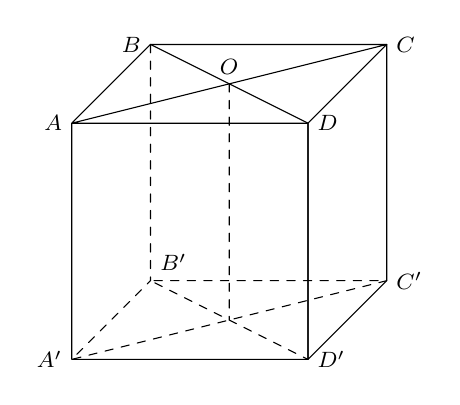
\begin{tikzpicture}[scale=0.5, font=\footnotesize, line join=round, line cap=round, >=stealth]
					\draw (0,0) node[left]{$A'$};
					\draw (2,2) node[above right]{$B'$};
					\draw (8,2) node[right]{$C'$};
					\draw (6,0) node[right]{$D'$};
					\draw (0,6) node[left]{$A$};
					\draw (2,8) node[left]{$B$};
					\draw (8,8) node[right]{$C$};
					\draw (6,6) node[right]{$D$};
					\draw (4,7) node[above]{$O$};
					\draw (0,0)--(0,6)--(6,6)--(6,0)--(0,0)(0,6)--(2,8)--(8,8)--(6,6)--(0,6)--(8,8);
					\draw (2,8)--(6,6)--(6,0) (8,8)--(8,2)--(6,0);
					\draw[dashed] (2,8)--(2,2)--(0,0)--(8,2)--(2,2)--(6,0) (4,7)--(4,1);
				\end{tikzpicture}
			}
			\item[b)] Ta có $(AA'D'D)\parallel (BB'C'C)$ suy ra \\
			$\mathrm{d}((AA'D'D),(BB'C'C))=\mathrm{d}(A,(BB'C'C))$.\\
			Do $AB\perp BB'$ và $AB\perp BC$, suy ra $AB\perp (BB'C'C)$.\\
			Vậy $\mathrm{d}((AA'D'D),(BB'C'C))=AB=a$.
		\end{enumerate}
	}
\end{vd}\dongcham{18}


\begin{dang}{Đoạn vuông góc chung. Khoảng cách giữa hai đường thẳng chéo nhau}
	\indamm{Dựng đoạn vuông góc chung:}
	\begin{itemize}
		\item [\iconMT] \indam{Trường hợp 1:}
		\immini{		
			Giả sử $a$ và $b$ là hai đường thẳng chéo nhau và $a \perp b$.
			\begin{itemize}
				\item[$\bullet$] Ta dựng mặt phẳng $(\alpha)$ chứa $a$ và vuông góc với $b$ tại $B$.
				\item[$\bullet$] Trong $(\alpha)$ dựng $BA \perp a$ tại $A$, ta được độ dài đoạn $AB$ là khoảng cách giữa hai đường thẳng chéo nhau $a$ và $b$.
			\end{itemize}
		}{
			\begin{tikzpicture}[scale=1, font=\footnotesize, line join=round, line cap=round,>=stealth]
				\tkzDefPoints{0/0/M,5/0/N,1.5/2.5/Q,6.5/2.5/P,2.5/-0.5/R,2.5/3.5/S,2.5/1.7/B,1.8/0.4/E,6/2.2/F}
				\tkzDefPointBy[homothety = center F ratio 0.4](E) \tkzGetPoint{A}
				\tkzInterLL(M,N)(R,S) \tkzGetPoint{I}
				\tkzDrawSegments(M,N N,P P,Q Q,M R,I B,S E,F A,B)
				\tkzDrawSegments[dashed](I,B)
				\tkzMarkAngles[size=1](N,M,Q)
				\tkzLabelAngles[color=black,pos=.6](Q,M,N){$\alpha$}
				\tkzLabelSegment[pos=0.9,right](R,S){$b$}
				\tkzLabelSegment[pos=0.9](E,F){$a$}
				\tkzMarkRightAngles[size=.3](B,A,F S,B,A)
				\tkzDrawPoints[fill=black](A,B)
				\tkzLabelPoints(A)
				\tkzLabelPoints[left](B)
			\end{tikzpicture}
		}
		\item [\iconMT] \indam{Trường hợp 2:}
		\immini{
			Giả sử $a$ và $b$ là hai đường thẳng chéo nhau nhưng không vuông góc với nhau.
			\begin{itemize}
				\item [$\bullet$] Ta dựng mặt phẳng $(\alpha)$ chứa $a$ và song song với $b$.
				\item [$\bullet$] Lấy một điểm $M$ tùy ý trên $b$ và dựng $MM'$ vuông góc với $(\alpha)$ tại $M'$.
				\item [$\bullet$] Từ $M'$ dựng $b'$ song song với $b$ cắt $a$ tại $A$.
			\end{itemize}
		}{
			\begin{tikzpicture}[scale=1, font=\footnotesize, line join=round, line cap=round,>=stealth]
				\tkzDefPoints{0/0/O,5/0/N,1.5/2.5/Q,6.5/2.5/P,1.6/3.5/R,5.5/3.5/S,1.6/1.8/E,4.7/3.5/M,4.7/1.8/M',2/2.3/G,4.8/0.2/H}
				\tkzDefPointBy[translation = from R to S](E) \tkzGetPoint{F}
				\tkzInterLL(G,H)(E,F) \tkzGetPoint{A}
				\tkzDefPointBy[translation = from M' to M](A) \tkzGetPoint{B}
				\tkzInterLL(P,Q)(A,B) \tkzGetPoint{J}
				\tkzInterLL(P,Q)(M,M') \tkzGetPoint{K}
				\tkzDrawSegments(O,N N,P P,K J,Q Q,O A,B M,M' R,S E,F G,H)
				\tkzDrawSegments[dashed](J,K)
				\tkzMarkAngles[size=1](N,O,Q)
				\tkzLabelAngles[color=black,pos=.6](Q,O,N){\normalsize $\alpha$}
				\tkzLabelSegment[pos=0.1,above](R,S){\normalsize $b$}
				\tkzLabelSegment[pos=0.9,above](G,H){\normalsize $a$}
				\tkzMarkRightAngles[size=.3](B,A,H A,B,M)
				\tkzDrawPoints[fill=black](A,B,M,M')
				\tkzLabelPoints[above](B,M)
				\tkzLabelPoints[below](A,M')
			\end{tikzpicture}
		}
		\begin{itemize}
		\item [$\bullet$] Từ $A$ dựng $AB$ song song với $MM'$ cắt $b$ tại $B$, độ dài đoạn $AB$ là khoảng cách giữa hai đường thẳng chéo nhau $a$ và $b$.
	\end{itemize}
	\end{itemize}
	\begin{luuy}
		\indam{Nhận xét:}
		\begin{itemize}
			\item Khoảng cách giữa hai đường thẳng chéo nhau bằng khoảng cách giữa một trong hai đường thẳng đó và mặt phẳng song song với nó chứa đường thẳng còn lại.
			\item Khoảng cách giữa hai đường thẳng chéo nhau bằng khoảng cách giữa hai mặt phẳng song song lần lượt chứa hai đường thẳng đó.
		\end{itemize}
	\end{luuy}
\end{dang}

\begin{vd}
	Cho tứ diện $OABC$ có $OA$, $OB$, $OC$ vuông góc với nhau đôi một và $OA = OB = OC = a$. Gọi $I$ là trung điểm của $BC$. Hãy dựng và tính độ dài đoạn vuông góc chung của
	\begin{enumEX}{2}
		\item $OA$ và $BC$.
		\item $AI$ và $OC$.
	\end{enumEX}
	\loigiai{
		\begin{center}
			\begin{tikzpicture}[scale=.8, font=\footnotesize, line join=round, line cap=round,>=stealth]
				\tkzDefPoints{0/0/O,0/5/A,4/-3/B,7/0/C}
				\tkzDefMidPoint(B,C) \tkzGetPoint{I}
				\tkzDefMidPoint(O,B) \tkzGetPoint{K}
				\tkzDefPointBy[homothety = center A ratio 0.6](K) \tkzGetPoint{H}
				\tkzDefPointBy[homothety = center A ratio 0.6](I) \tkzGetPoint{E}
				\tkzDefPointBy[translation = from H to O](E) \tkzGetPoint{F}
				\tkzDrawSegments(O,A O,B B,C A,K A,B A,I A,C O,H)
				\tkzDrawSegments[dashed](O,C K,I H,E E,F O,I)
				\tkzMarkRightAngles[size=.3](A,O,B A,O,C B,O,C O,H,K F,E,I E,F,C I,K,B)
				\tkzDrawPoints[fill=black](A,B,C,O,I,K,H,E,F)
				\tkzLabelPoints[above](A)
				\tkzLabelPoints[below](B)    		
				\tkzLabelPoints[right](E,I,C)
				\tkzLabelPoints[left](O,H)
				\tkzLabelPoints[below left](K)
				\tkzLabelPoints[below right](F)
			\end{tikzpicture}
		\end{center}
		\begin{enumerate}[a)]
			\item Ta có $\heva{&OA \perp OI\\ &BC \perp OI}$ $\Rightarrow OI$ là đoạn vuông góc chung của $OA$ và $BC$.\\
			Tam giác $OBC$ vuông cân tại $O$ nên $OI = \dfrac{BC}{2} = \dfrac{a\sqrt{2}}{2}$.\\
			Vậy $\mathrm{d}(OA, BC) = \dfrac{a\sqrt{2}}{2}$.
			\item Gọi $K$ là trung điểm của $OB$, ta có $IK \parallel OC$ $\Rightarrow OC \parallel (AIK)$.\\
			Ta có $\heva{&IK \perp OB\\ &IK \perp OA}$ $\Rightarrow IK \perp (OAB)$ $\Rightarrow (AIK) \perp (OAB)$ theo giao tuyến $AK$.\\
			Trong mặt phẳng $(OAB)$, kẻ $OH \perp AK$ tại $H$, ta có: $OH \perp (AIK)$ $\Rightarrow OH \perp AI$.\\
			Trong mặt phẳng $(AIK)$, kẻ $HE \parallel IK$ $(E \in SI)$.\\
			Trong mặt phẳng $(HE, OC)$, kẻ $EF \parallel OH$ $(F \in OC)$ $\Rightarrow EF \perp AI$.\\
			Lại có $OC \perp (OAB) \Rightarrow OC \perp AH \Rightarrow OC \perp EF$. Do đó $EF$ là đoạn vuông góc chung của $OC$ và $AI$.\\
			Trong tam giác vuông $OAK$ ta có: $\dfrac{1}{OH^2} = \dfrac{1}{OA^2} + \dfrac{1}{OK^2} = \dfrac{1}{a^2} + \dfrac{4}{a^2} = \dfrac{5}{a^2}$.\\
			Suy ra $EF = OH = \dfrac{a\sqrt{5}}{5}$. Vậy $\mathrm{d}(AI, OC) = \dfrac{a\sqrt{5}}{5}$.
		\end{enumerate}
	}
\end{vd}\dongcham{24}

\begin{vd}
	Cho hình lăng trụ đứng $ABC.A'B'C'$ có đáy $ABC$ là tam giác vuông tại $A$ với $AB = a$, $AC = 2a$; cạnh bên $AA' = 2a$. Hãy dựng và tính độ dài đoạn vuông góc chung của hai đường thẳng $BC'$ và $AA'$.
	\loigiai{
		\immini{
			Ta có $AA' \parallel BB'$ $\Rightarrow AA' \parallel (BB'C'C)$.\\
			Vì $(A'B'C') \perp (BB'C'C)$ theo giao tuyến $B'C'$ nên trong mặt phẳng $(A'B'C')$, kẻ $A'H \perp B'C'$ tại $H$, ta có: $A'H \perp (BB'C'C)$ $\Rightarrow A'H \perp BC'$.\\
			Trong mặt phẳng $(BB'C'C)$, kẻ $HF \parallel AA'$ $(F \in BC')$.
			Trong mặt phẳng $(HF, AA')$, kẻ $FE \parallel A'H$ $(E \in AA')$ $\Rightarrow FE \perp BC'$.\\
			Ta có $AA' \perp (A'B'C') \Rightarrow AA' \perp A'H \Rightarrow AA' \perp FE$.\\
			Do đó $EF$ là đoạn vuông góc chung của $AA'$ và $BC'$.\\
			Trong tam giác vuông $A'B'C'$ ta có: $$\dfrac{1}{A'H^2} = \dfrac{1}{A'B'^2} + \dfrac{1}{A'C'^2} = \dfrac{1}{a^2} + \dfrac{1}{4a^2} = \dfrac{5}{4a^2}.$$
			Suy ra $EF = A'H = \dfrac{2a\sqrt{5}}{5}$.\\
			Vậy $\mathrm{d}(AA', BC') = \dfrac{2a\sqrt{5}}{5}$.
		}{
			\begin{tikzpicture}[scale=.6, font=\footnotesize, line join=round, line cap=round,>=stealth]
				\tkzDefPoints{0/0/A,2/-3/B,6/0/C,0/7/A'}
				\tkzDefPointBy[translation = from A to A'](B) \tkzGetPoint{B'}
				\tkzDefPointBy[translation = from A to A'](C) \tkzGetPoint{C'}
				\tkzDefPointBy[homothety = center B' ratio 0.4](C') \tkzGetPoint{H}
				\tkzDefPointBy[homothety = center B ratio 0.4](C') \tkzGetPoint{F}
				\tkzDefPointBy[translation = from H to F](A') \tkzGetPoint{E}
				\tkzDrawSegments(A,B B,C A,A' A',B' B',C' A',C' A',H H,F B,C' B,B' C,C')
				\tkzDrawSegments[dashed](A,C E,F)
				\tkzMarkRightAngles[size=.3](B',A',C' A',H,B' A',E,F E,F,B A,A',B')
				\tkzDrawPoints[fill=black](A,B,C,A',B',C',H,E,F)
				\tkzLabelPoints[above left](A')
				\tkzLabelPoints[above right](C')
				\tkzLabelPoints[below](B)    		
				\tkzLabelPoints[right](C,F)
				\tkzLabelPoints[left](A,E)
				\tkzLabelPoints[below left](B')    
				\tkzLabelPoints(H)	
			\end{tikzpicture}
		}
	}
\end{vd}\dongcham{24}

\begin{vd}
	Cho hình chóp $S.ABCD$ có đáy là hình vuông cạnh bằng $a$, $SA$ vuông góc với đáy và $SA = a$. $M$ là trung điểm của $SB$. Tính khoảng cách giữa các đường thẳng
	\begin{enumEX}{3}		
		\item $SC$ và $BD$.
		\item $AC$ và $SD$.
		\item $SD$ và $AM$.
	\end{enumEX}
	\loigiai{
		\begin{center}
			\begin{tikzpicture}[line join=round,scale=0.7]
				\tkzDefPoints{0/0/A,-3/-3/D,3/-3/C,6/0/B,0/5/S}
				\tkzDefMidPoint(S,B) \tkzGetPoint{M}
				\tkzInterLL(A,C)(B,D) \tkzGetPoint{O}
				\tkzDefPointBy[translation = from C to D](A) \tkzGetPoint{E}		
				\tkzDefPointBy[translation = from O to D](A) \tkzGetPoint{I}
				\tkzDefPointBy[homothety = center S ratio 0.7](C) \tkzGetPoint{H}
				\tkzDefPointBy[homothety = center S ratio 0.6](I) \tkzGetPoint{K}
				\tkzDrawSegments(S,E S,D S,C S,B C,D B,C M,C D,E S,I)
				\tkzDrawSegments[dashed](S,A A,D A,B A,K A,E A,M O,M O,H A,C B,D A,I)
				\tkzMarkRightAngles[size=.3](S,A,B S,A,D B,A,D A,I,D A,K,I O,H,C D,O,H)
				\tkzDrawPoints[fill=black](A,B,C,D,E,S,I,O,M,H,K) 
				\tkzLabelPoints(C)
				\tkzLabelPoints[above](S)
				\tkzLabelPoints[below](O)    		
				\tkzLabelPoints[right](H,B)
				\tkzLabelPoints[left](E,K,I)
				\tkzLabelPoints[below left](D)
				\tkzLabelPoints[above left](A)
				\tkzLabelPoints[above right](M)
			\end{tikzpicture}
		\end{center}
		\begin{enumerate}
			\item Gọi $O$ là giao điểm của $AC$ và $BD$. Ta có: $\heva{&BD \perp SA\\ &BD \perp AC}$ $\Rightarrow BD \perp (SAC)$ tại $O$.\\
			Trong mặt phẳng $(SAC)$, kẻ $OH \perp SC$ tại $H$, ta có $OH \perp SC$ và $OH \perp BD$ (vì $BD \perp (SAC)$).\\
			Vậy $OH$ là đoạn vuông góc chung của $BD$ và $SC$.\\
			Ta có $\dfrac{OH}{OC} = \dfrac{SA}{SC} = \sin \widehat{ACS}$ $\Rightarrow OH = \dfrac{OC.SA}{SC} = \dfrac{\dfrac{a\sqrt{2}}{2}\cdot a}{a\sqrt{3}} = \dfrac{a\sqrt{6}}{6}$.\\
			Vậy $\mathrm{d}(SC, BD) = OH = \dfrac{a\sqrt{6}}{6}$.
			\item Dựng hình bình hành $ACDE$, ta có: $AC \parallel DE$ $\Rightarrow AC \parallel (SDE)$.\\
			$\Rightarrow \mathrm{d}(AC, SD) = \mathrm{d}(AC, (SDE)) = \mathrm{d}(A, (SDE))$.\\
			Trong mặt phẳng $(ABCD)$, kẻ $AI \perp DE$ tại $I$, ta có $\heva{&DE \perp AI\\ &DE \perp SA}$ $\Rightarrow DE \perp (SAI)$.\\
			$\Rightarrow (SDE) \perp (SAI)$ theo giao tuyến $SI$.\\
			Trong mặt phẳng $(SAI)$, kẻ $AK \perp SI$ tại $K$, ta có: $AK \perp (SDE)$ $\Rightarrow AK = \mathrm{d}(A, (SDE))$.\\
			Ta có $AIDO$ là hình bình hành nên $AI = OD = \dfrac{a\sqrt{2}}{2}$.\\
			Trong tam giác vuông $SAI$ ta có: $\dfrac{1}{AK^2} = \dfrac{1}{AI^2} + \dfrac{1}{SA^2} = \dfrac{2}{a^2} + \dfrac{1}{a^2} = \dfrac{3}{a^2}$.\\
			Suy ra $AK = \dfrac{a\sqrt{3}}{3}$.\\
			Vậy $\mathrm{d}(AC, SD) = \mathrm{d}(A, (SDE)) = AK = \dfrac{a\sqrt{3}}{3}$.
			\item Ta có $OM \parallel SD$ và $AC \parallel DE$ nên $(AMC) \parallel (SDE)$.\\
			Suy ra $\mathrm{d}(SD, AM) = \mathrm{d}((AMC), (SDE)) = \mathrm{d}(A, (SDE)) = AK = \dfrac{a\sqrt{3}}{3}$.
		\end{enumerate}
	}
\end{vd}\dongcham{39}

\begin{vd}%[1H2B5-4]
	Cho hình lập phương $ABCD.A'B'C'D'$ cạnh $a$. Gọi $M$, $N$ lần lượt là trung điểm của $AC$ và $B'C'$. Tính khoảng cách giữa hai đường thẳng $MN$ và $B'D'$.
	\loigiai{
		\immini{$B'D'$ cắt $A'C'$ tại $O$. Gọi $P$ là trung điểm của $OC$.\\
			Vẽ $OH \perp MP$, $HE\parallel NP$, $EF\parallel OH$.\\
			Ta có $\mathrm{d}\left(MN, B'D'\right)=EF=OH$.\\
			Xét tam giác vuông $MOP$, ta có $OM=a$, $OP=\dfrac{a \sqrt{2}}{4}$, suy ra $OH=\dfrac{a}{3}$.}
		{\begin{tikzpicture}[scale=0.7, font=\footnotesize, line join=round, line cap=round, >=stealth]
				\path
				(0,0) coordinate (B) 
				(4,0) coordinate (C) 
				(1.5,1.5) coordinate (A) 
				(A)+(4,0) coordinate (D);
				\foreach \x in {A,B,C,D}
				\path (\x)+(0,-3.5) coordinate(\x');
				\path
				($(A)!.5!(C)$) coordinate (M)
				($(B')!.5!(C')$) coordinate (N)
				($(A')!.5!(C')$) coordinate (O)
				($(O)!.5!(C')$) coordinate (P)
				($(M)!.75!(P)$) coordinate (H)
				($(M)!.75!(N)$) coordinate (E)
				($(B')!.65!(O)$) coordinate (F);
				\draw[dashed] (B')--(A')--(D')--(B') (A)--(A')--(C') (M)--(N)--(P)--(M) (E)--(H)--(O)--(M) (E)--(F);
				\draw (B')--(C')--(D')--(D)--(A)--(B)--(C)--(D) (A)--(C)--(C') (B)--(B');
				\foreach \p/\g in {B/180,C/0,D/0,A/180,B'/180,C'/0,D'/0,A'/160,O/-90,P/0,M/90,N/-90,H/0,E/180,F/180}\draw[fill=black] (\p) circle (1pt)node[shift={(\g:.3)}]{$\p$};
		\end{tikzpicture}}	
	}
\end{vd}\dongcham{19}

\begin{vd}%[1H2K5-4]
	Cho tứ diện đều $ABCD$ có cạnh bằng $\sqrt{11}$. Gọi $I$ là trung điểm của cạnh $CD$. Tính khoảng cách giữa hai đường thẳng $AC$ và $BI$.
	\loigiai{
		\immini{Gọi $O$ là trung điểm $AC$, $J$ là trung điểm $OD$.\\
			Vẽ $OH \perp BJ$, $HE\parallel AC$, $EF\parallel OH$.\\
			Ta có $\mathrm{d}(AC, BJ)=EF=OH$.\\
			Xét tam giác $OBD$ cân tại $O$, ta có
			$BD=\sqrt{11}$, $OB=OD=\dfrac{\sqrt{33}}{2}, BJ=\dfrac{\sqrt{11}}{4}$,
			$S_{\triangle OBD}=\dfrac{11 \sqrt{2}}{4}$, $OH=\sqrt{2}$.}
		{\begin{tikzpicture}[font=\footnotesize, line join=round, line cap=round, >=stealth,scale=.8]
				\path 	(0:0) coordinate (B)
				++(0:5) coordinate (D)
				++(-150:4) coordinate (C)
				($(D)!0.5!(C)$) coordinate (M)
				($(B)!2/3!(M)$) coordinate (G)
				($(G)+(95:4.5)$) coordinate (A)
				($(D)!0.5!(C)$) coordinate (I)
				($(A)!0.5!(C)$) coordinate (O)
				($(O)!0.5!(D)$) coordinate (J)
				($(B)!0.65!(J)$) coordinate (H)
				($(B)!0.65!(I)$) coordinate (E)
				($(C)!0.65!(O)$) coordinate (F)
				;
				\draw (D)--(C)--(B)--(A)--(C) (B)--(O)--(D)--(A) (I)--(J); 
				\draw[dashed] (J)--(B)--(D) (O)--(H)--(E)--(F) (B)--(I);
				\foreach \x / \goc in {B/180,C/-90,D/0,O/150,A/90,I/-90,J/90,H/75,E/-90,F/200}\fill (\x) circle (1pt) ($(\x)+(\goc:3mm)$) node[scale=.8]{$\x$};
		\end{tikzpicture}}
	}
\end{vd}\dongcham{19}


